\documentclass[12pt,letterpaper]{article}
\usepackage[utf8]{inputenc}
\usepackage[margin=1in]{geometry}
\usepackage{graphicx}
\usepackage{fancyhdr}
\usepackage[hidelinks]{hyperref}

% Header and footer
\pagestyle{fancy}
\fancyhf{}
\fancyhead[C]{\textbf{Certified Translation - Patrika}}
\fancyfoot[C]{Page \thepage}
\renewcommand{\headrulewidth}{0.4pt}
\renewcommand{\footrulewidth}{0.4pt}

\begin{document}

\begin{center}
\textbf{\Large CERTIFIED TRANSLATION}\\[0.3cm]
\rule{\textwidth}{1.5pt}\\[0.3cm]
\textbf{\large English Translation of Hindi Newspaper Article}\\[0.2cm]
\rule{\textwidth}{1.5pt}
\end{center}

\vspace{0.5cm}

\noindent\textbf{Source Document Information:}
\begin{itemize}
    \setlength\itemsep{0.2em}
    \item \textbf{Publication:} Patrika (पत्रिका)
    \item \textbf{Original Language:} Hindi (Devanagari script)
    \item \textbf{Date of Publication:} December 2024
    \item \textbf{Article Title:} ``आनंद इंटरनेशनल कॉलेज में विशेष व्याख्यान कंप्यूटर साइंस क्षेत्र में करियर के अवसरों पर दिया मार्गदर्शन'' \\
    (``Special Lecture on Career Opportunities in Computer Science at Anand International College'')
    \item \textbf{Location:} Jaipur, Rajasthan, India
\end{itemize}

\vspace{0.5cm}

\section*{ORIGINAL HINDI ARTICLE (IMAGE)}

\begin{center}
\fbox{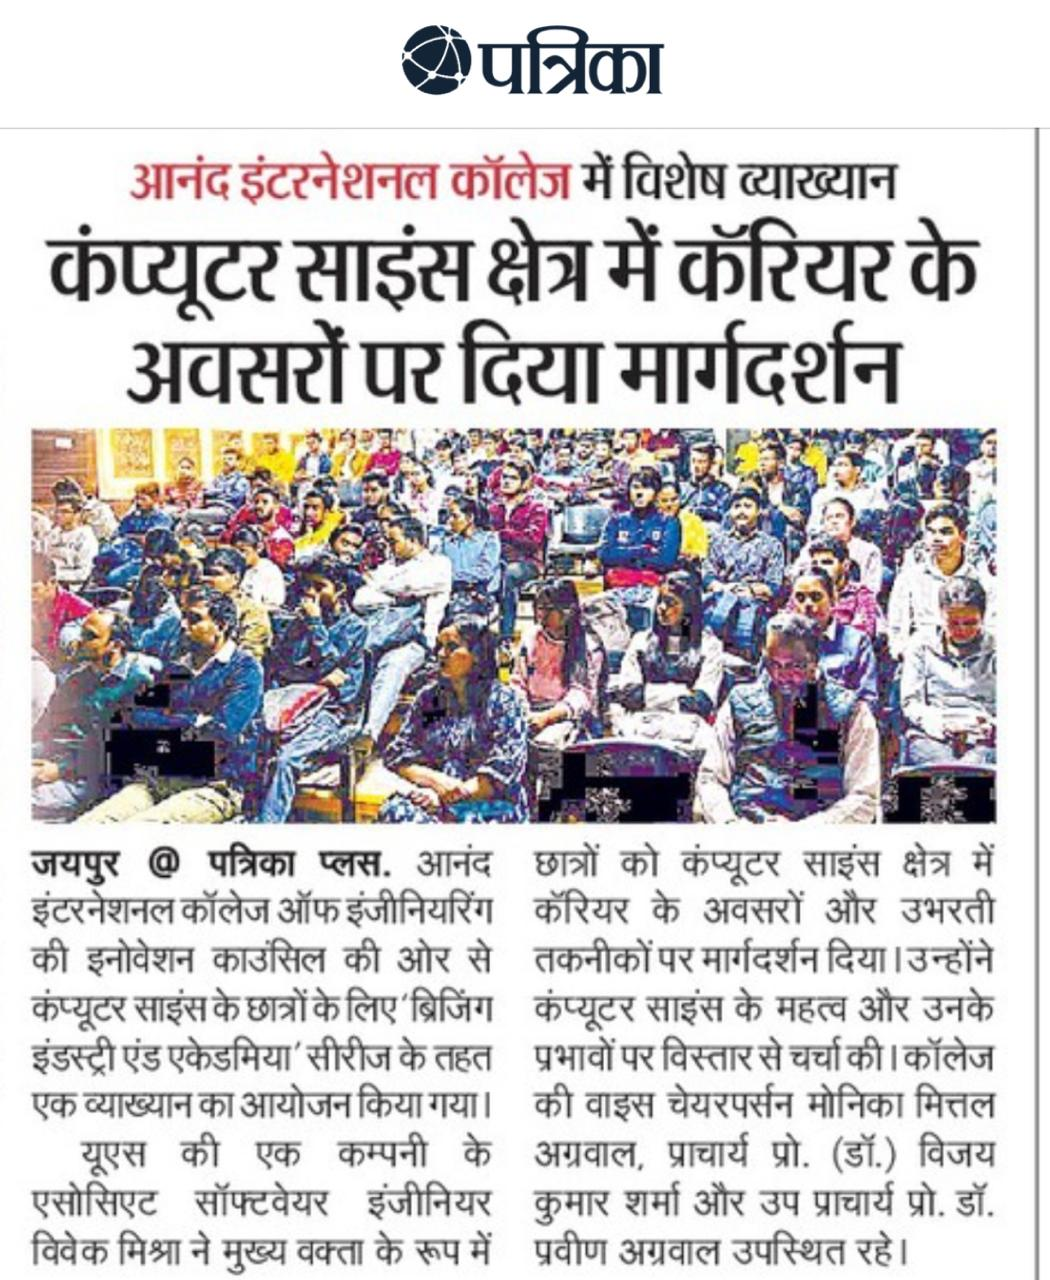
\includegraphics[width=0.95\textwidth]{../WhatsApp Image 2024-12-08 at 08.31.21.jpeg}}
\end{center}

\vspace{0.5cm}

\section*{CERTIFIED ENGLISH TRANSLATION}

\subsection*{Special Lecture on Career Opportunities in Computer Science at Anand International College}

\noindent\textbf{JAIPUR @ PATRIKA PLUS:} Under the Innovation Council of Anand International College of Engineering, a special lecture was organized for Computer Science students on the topic of ``Bridging Industry and Academia'' Hybrid Lecture Series. As the chief speaker, Vivek Mishra, an Associate Software Engineer from JPMorgan Chase \& Co., a US-based company, shared extensive information with students about future-oriented techniques and the significance of Computer Science. He discussed Computer Science significance and its various applications in detail. Students asked several valuable questions during the session. College Vice Chairperson Monika Mittal Agrawal, Principal Prof. (Dr.) Vijay Kumar Sharma, and Vice Principal Prof. (Dr.) Praveen Agrawal were present on this occasion.

\vspace{1cm}

\noindent\rule{\textwidth}{1.5pt}

\section*{TRANSLATOR'S CERTIFICATION STATEMENT}

\noindent I, \textbf{Subhash K Chand}, hereby certify that:

\begin{enumerate}
    \item I am competent and fluent in both the \textbf{Hindi} (Devanagari script) and \textbf{English} languages.
    
    \item I possess the necessary qualifications and linguistic ability to translate documents from Hindi to English accurately and completely.
    
    \item The above English translation is a \textbf{complete, accurate, and faithful} translation of the original Hindi newspaper article published in Patrika newspaper.
    
    \item I have personally reviewed both the original Hindi article (image shown above) and this English translation to ensure accuracy and completeness.
    
    \item I have the ability to \textbf{read, write, and comprehend} both Hindi and English languages at a professional level.
    
    \item This translation captures the full meaning and intent of the original article to the best of my professional ability.
\end{enumerate}

\vspace{0.8cm}

\noindent\textbf{Translator's Signature:} \rule{7cm}{0.4pt}

\vspace{0.5cm}

\noindent
\begin{tabular}{ll}
\textbf{Name:} & Subhash K Chand \\[0.3cm]
\textbf{Professional Title:} & Certified Translator (Hindi-English) \\[0.3cm]
\textbf{LinkedIn Profile:} & linkedin.com/in/subhashkchand \\[0.3cm]
\textbf{Contact Information:} & \rule{6cm}{0.4pt} \\[0.3cm]
\textbf{Date of Certification:} & January 19, 2026 \\
\end{tabular}

\vspace{1cm}

\noindent\rule{\textwidth}{1.5pt}

\vspace{0.3cm}

\begin{center}
\textit{\small This certification is provided in accordance with U.S. Citizenship and Immigration Services (USCIS) requirements for certified translations of foreign language documents as outlined in 8 CFR § 103.2(b)(3). The translator affirms competence in both source and target languages and attests to the accuracy and completeness of this translation.}
\end{center}

\end{document}
